% !TEX program = pdflatex
\documentclass[12pt]{article}

\IfFileExists{spanish.ldf}{
    \usepackage[spanish]{babel}
}{
    \usepackage{babel}
    \renewcommand{\figurename}{Figura}
    \renewcommand{\tablename}{Tabla}
}
\usepackage[utf8]{inputenc}
\usepackage[T1]{fontenc}

\IfFileExists{newtxtext.sty}{\usepackage{newtxtext,newtxmath}}{}
\usepackage[a4paper,margin=2.5cm]{geometry}
\IfFileExists{setspace.sty}{\usepackage{setspace}}{}
\usepackage{graphicx}
\usepackage{amsmath}
\usepackage{float}
\usepackage[hidelinks]{hyperref}
\IfFileExists{xurl.sty}{\usepackage{xurl}}{}
\usepackage{booktabs}
\usepackage{array}
\usepackage{longtable}
\usepackage{tabularx}

\IfFileExists{setspace.sty}{\setstretch{1.15}}{\linespread{1.15}}
\renewcommand{\arraystretch}{1.15}
\graphicspath{{../capturas/}{./}}
\setlength{\emergencystretch}{3em}

\begin{document}

\hypersetup{pageanchor=false}
\begin{titlepage}
\thispagestyle{empty}
\vspace*{1.2cm}

\begin{center}
{\Large \textbf{UNIVERSIDAD DEL VALLE DE GUATEMALA}}\\[0.4cm]
{\normalsize Facultad de Ingeniería}\\
{\normalsize Redes}\\
{\normalsize Semestre II -- 2026}\\[1.2cm]


\includegraphics[width=0.42\textwidth]{logo.png}\\[1.4cm]

{\LARGE \textbf{Proyecto 1}}\\[0.3cm]
{\Large Uso de un protocolo existente}\\[0.3cm]
\end{center}

\vfill

\begin{flushright}
\textbf{Integrantes:}\\
Nájera Marakovits, Ingrid Nina Alessandra -- 231088
\end{flushright}

\end{titlepage}
\hypersetup{pageanchor=true}
\pagenumbering{arabic}

\section*{Resumen}

El proyecto implementa un chatbot de consola que utiliza la API REST de Gemini y Model Context Protocol. El anfitrión mantiene el contexto de la conversación y coordina servidores para Filesystem, Git y operaciones de red. El cliente MCP, el servidor personalizado y los transportes local y remoto se implementaron manualmente con JSON-RPC 2.0.

El servidor de operaciones de red ofrece cuatro herramientas de diagnóstico de solo lectura. La versión local utiliza entrada y salida estándar. La versión remota utiliza MCP Streamable HTTP sobre HTTPS y se encuentra desplegada en Render. La comunicación remota fue capturada con Wireshark para analizar la sincronización, las solicitudes, las respuestas y las capas de red.

\section{Objetivos}

\begin{itemize}
    \item Conectar un chatbot con Gemini mediante su API REST.
    \item Mantener el contexto durante una sesión de conversación.
    \item Integrar los servidores oficiales Filesystem y Git.
    \item Desarrollar manualmente un servidor MCP para operaciones de red.
    \item Publicar el servidor mediante HTTPS en Render.
    \item Capturar y clasificar el tráfico MCP con Wireshark.
    \item Validar la solución con pruebas automatizadas y ejecuciones reales.
\end{itemize}

\section{Arquitectura y funcionamiento}

El archivo src/chatbot.py funciona como anfitrión. La comunicación con Gemini se realiza mediante solicitudes HTTP y la comunicación con los servidores MCP se realiza desde src/mcp\_client.py. El servidor personalizado se encuentra en src/network\_server.py y el transporte remoto en src/remote\_server.py.

\begin{table}[H]
\centering
\small
\begin{tabularx}{\textwidth}{|p{3.2cm}|p{2.8cm}|X|}
\hline
Componente & Transporte & Función \\
\hline
Gemini & HTTPS & Interpretar la solicitud y redactar la respuesta \\
\hline
Filesystem & Entrada y salida estándar & Operaciones controladas sobre archivos \\
\hline
Git & Entrada y salida estándar & Estado, preparación, commits e historial \\
\hline
Network local & Entrada y salida estándar & Diagnósticos de red locales \\
\hline
Network remoto & HTTPS & Diagnósticos desde el servicio en Render \\
\hline
\end{tabularx}
\caption{Componentes principales de la solución}
\end{table}

El flujo comienza cuando el usuario escribe una solicitud. El anfitrión guarda el mensaje en el historial y envía a Gemini solamente las herramientas relacionadas. Si Gemini solicita una función, la consola muestra el nombre y los argumentos. Luego de la confirmación, el cliente envía tools/call al servidor. El resultado vuelve a Gemini para producir la respuesta final.

El ciclo MCP utiliza initialize, notifications/initialized, tools/list y tools/call. Las solicitudes incluyen un identificador y las respuestas conservan el mismo valor. Las notificaciones no tienen identificador y no producen una respuesta JSON-RPC.

\section{Integración con Gemini}

La conexión utiliza el endpoint generateContent de Gemini. El historial conserva los mensajes del usuario, las respuestas del modelo y los resultados de herramientas. Una prueba real solicitó información sobre Alan Turing y luego preguntó el año de nacimiento. El modelo respondió 1912 al utilizar el contexto anterior.

El chatbot registra las interacciones en logs/mcp.jsonl. Cada entrada contiene fecha, servidor, dirección y mensaje. Los secretos se cargan desde .env, archivo excluido de Git. También se agregaron reintentos para errores temporales de Gemini y selección contextual de herramientas para reducir solicitudes innecesarias.

\section{Servidores oficiales}

El servidor Filesystem se limita al directorio del proyecto. El servidor Git trabaja sobre el repositorio actual. La demostración creó docs/mcp-demo/README.md, agregó únicamente ese archivo al área de preparación y generó un commit desde el servidor MCP Git. El estado final confirmó que ambas integraciones funcionaron correctamente.

\section{Servidor MCP de operaciones de red}

El servidor se identifica como uvg-network-operations y utiliza la versión MCP 2025-11-25. Su propósito es apoyar tareas de una mesa de ayuda mediante verificaciones pequeñas y de solo lectura.

\begin{table}[H]
\centering
\footnotesize
\begin{tabularx}{\textwidth}{|>{\raggedright\arraybackslash}p{3.6cm}|>{\raggedright\arraybackslash}p{4cm}|X|}
\hline
Herramienta & Entrada & Resultado \\
\hline
resolve\_dns & hostname e ip version opcional & Direcciones IP únicas \\
\hline
\shortstack[l]{check\_tcp\_\\connection} & host, puerto y tiempo opcional & Estado y tiempo de conexión \\
\hline
analyze\_cidr & Red en formato CIDR & Red, máscara, broadcast y rango útil \\
\hline
\shortstack[l]{get\_local\_\\network\_info} & Sin parámetros & Nombre del equipo y direcciones locales \\
\hline
\end{tabularx}
\caption{Herramientas del servidor personalizado}
\end{table}

Los argumentos se validan mediante esquemas JSON. Una entrada inválida devuelve un resultado con isError en verdadero sin detener el servidor. La ejecución de analyze\_cidr para 192.168.100.70/26 produjo la red 192.168.100.64/26, el broadcast 192.168.100.127 y 62 direcciones utilizables.

\section{Despliegue remoto}

La misma lógica se ejecuta en un contenedor Docker publicado en Render. El servicio utiliza un usuario sin privilegios, recibe el puerto mediante la variable PORT y requiere autenticación Bearer para MCP. El token no se almacena en el repositorio.

\begin{table}[H]
\centering
\small
\begin{tabularx}{\textwidth}{|p{2.5cm}|p{2.5cm}|p{3cm}|X|}
\hline
Endpoint & Método & Autenticación & Resultado \\
\hline
/health & GET & No & Estado, nombre y versión \\
\hline
/mcp & POST & Bearer & Solicitudes MCP mediante JSON \\
\hline
/mcp & GET & Bearer & Código 405 \\
\hline
/mcp & DELETE & Bearer & Código 405 \\
\hline
\end{tabularx}
\caption{Endpoints del servicio remoto}
\end{table}

El health check público respondió HTTP 200. El cliente remoto negoció la versión MCP, descubrió cuatro herramientas y ejecutó correctamente analyze\_cidr y resolve\_dns. La dirección del servicio es \href{https://uvg-network-operations.onrender.com}{https://uvg-network-operations.onrender.com}.

\section{Captura con Wireshark}

La comunicación utiliza TLS 1.3. Para observar JSON-RPC se guardaron temporalmente las claves de la sesión TLS del proceso de prueba. Wireshark utilizó esas claves para descifrar únicamente la conexión con Render. La captura se limitó al puerto 443 y produjo 91 paquetes. El archivo de captura y las claves permanecen fuera de Git.

\begin{figure}[H]
\centering
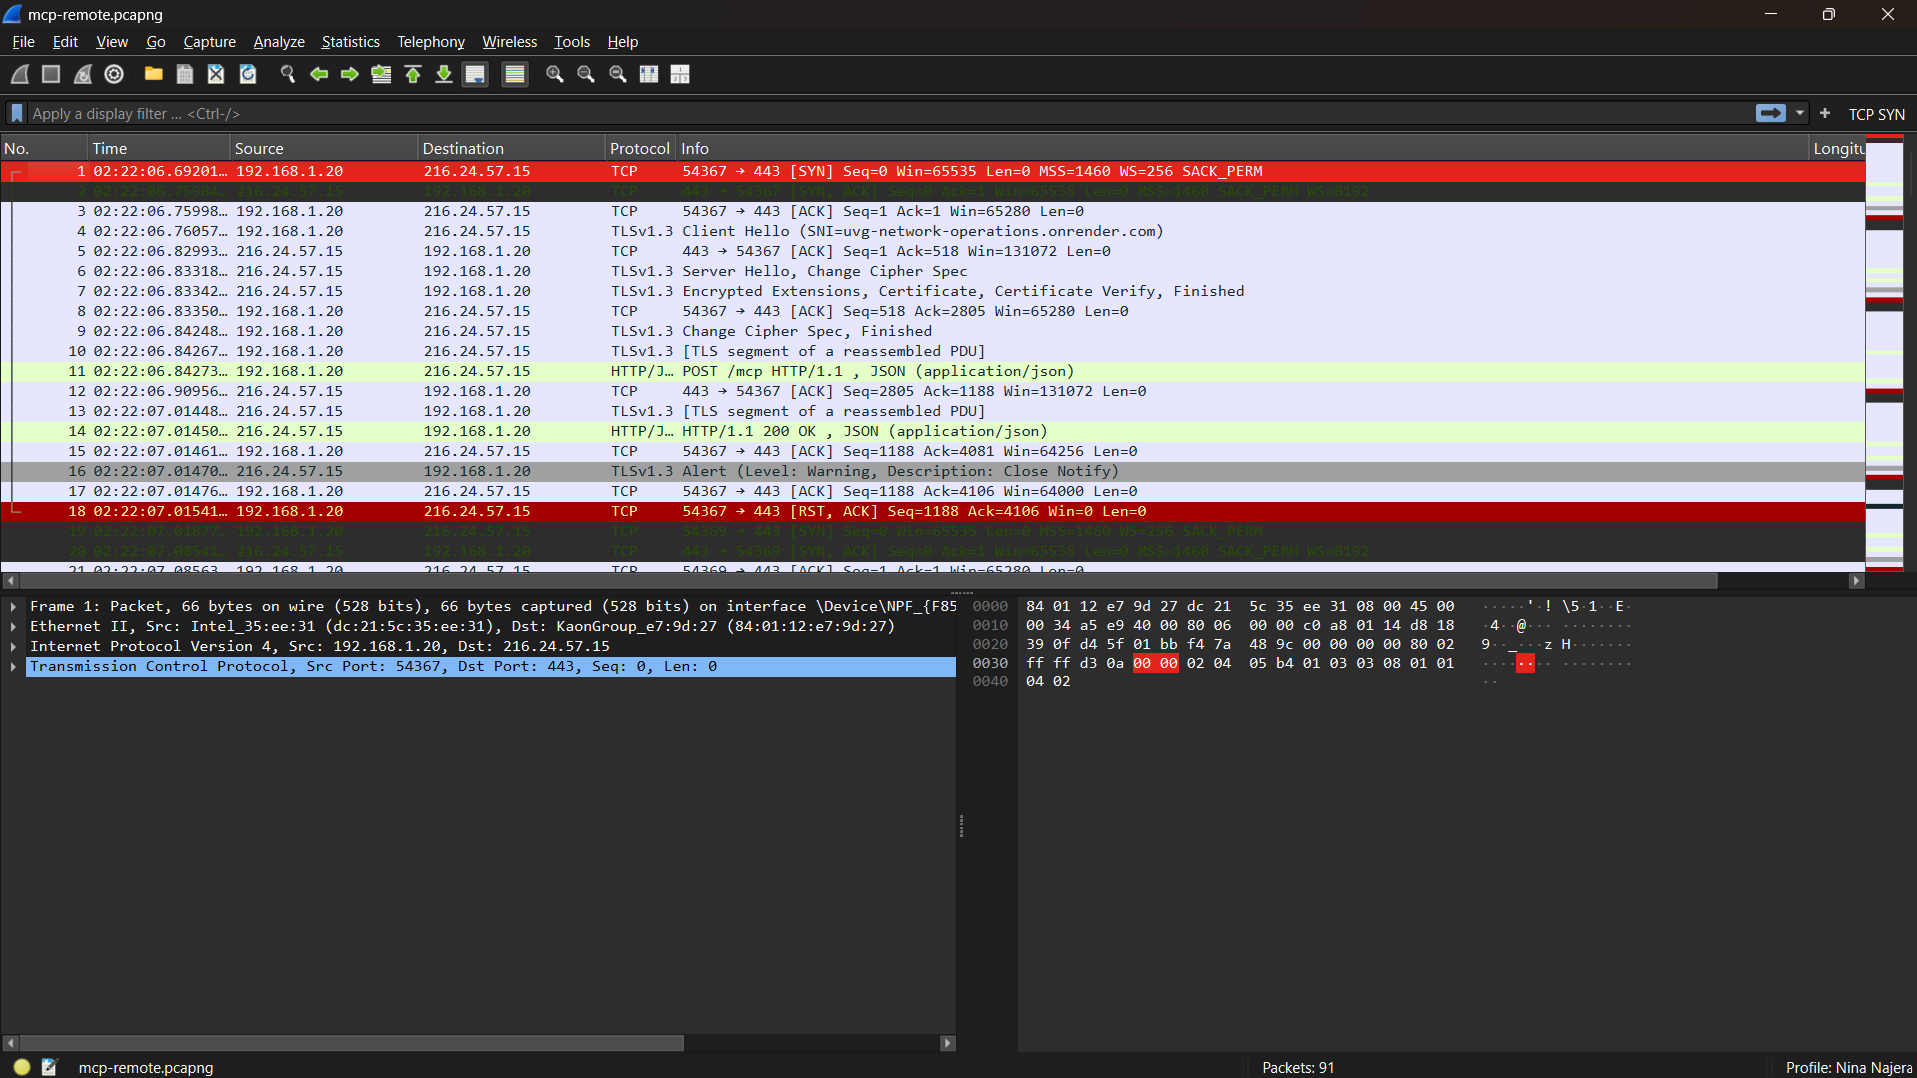
\includegraphics[width=0.94\textwidth]{01_tls_handshake_overview.png}
\caption{Establecimiento TCP y negociación TLS 1.3}
\end{figure}

\begin{figure}[H]
\centering
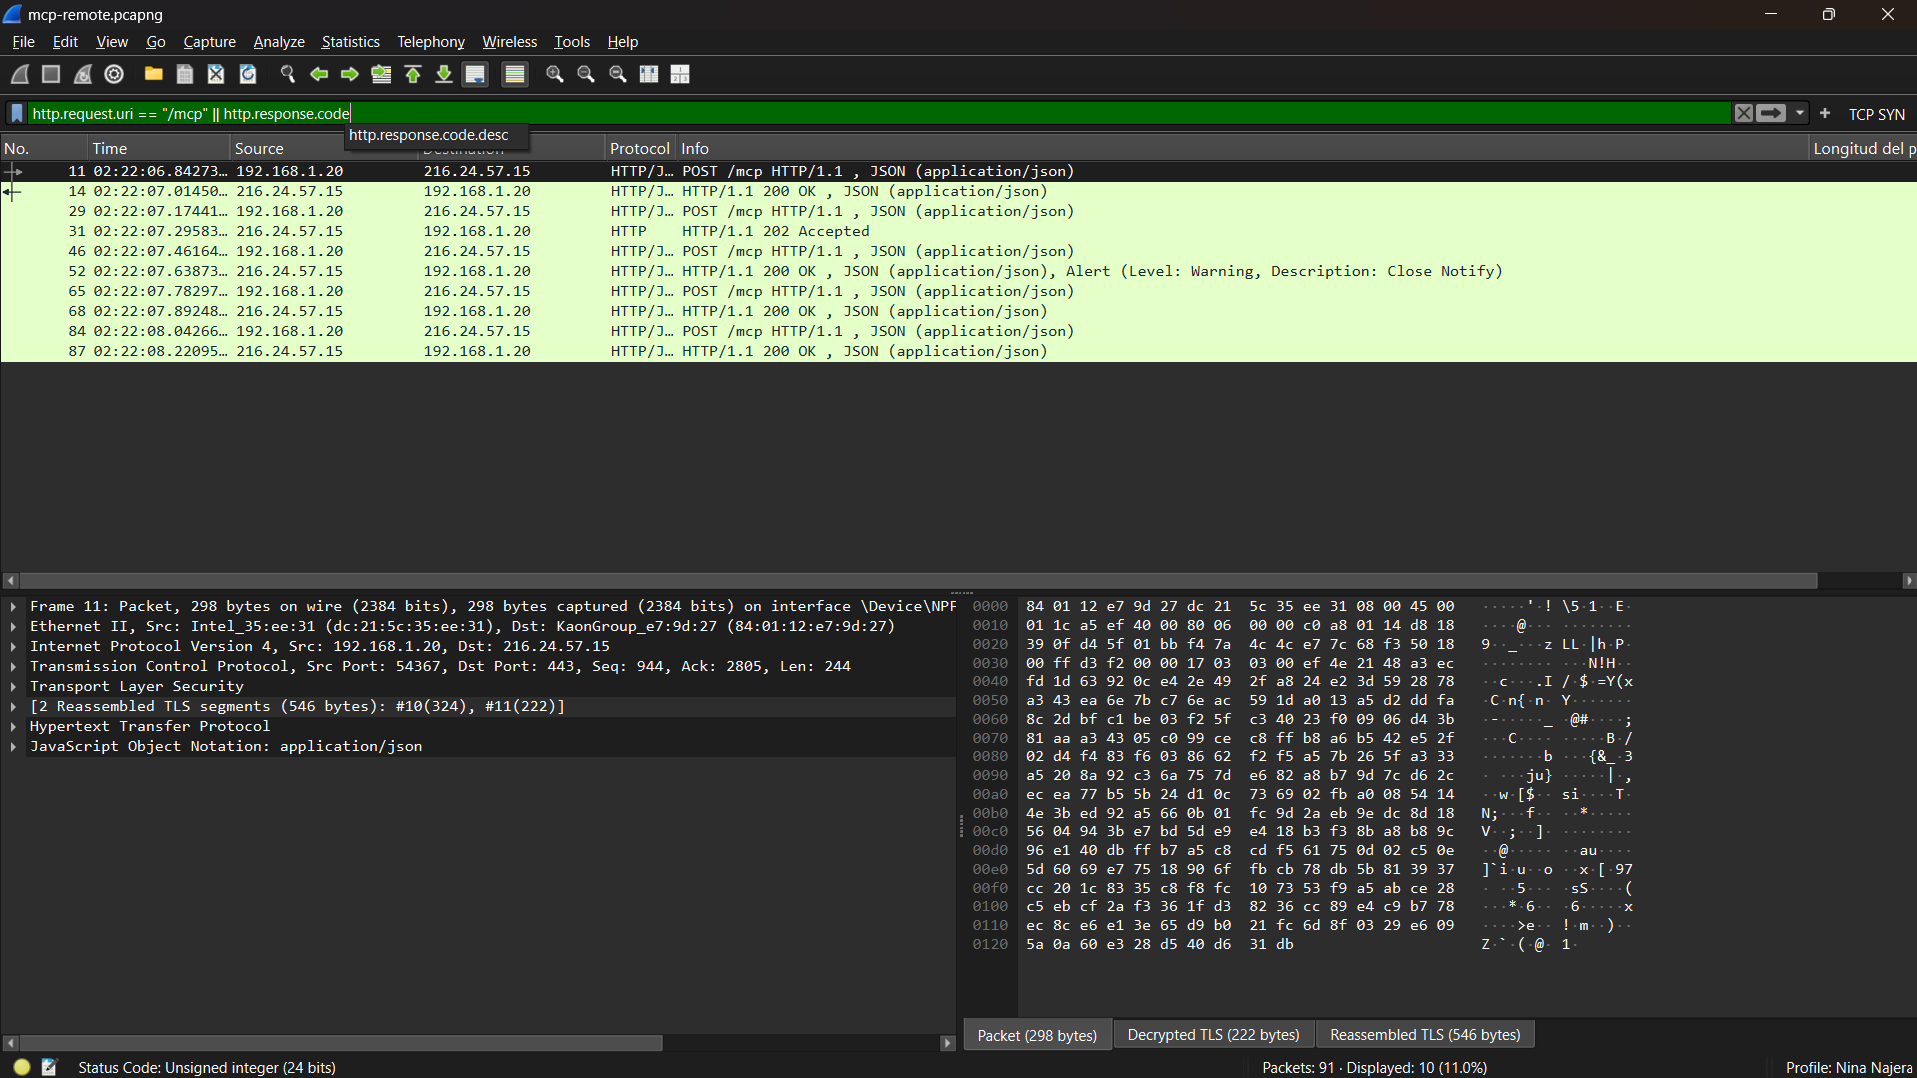
\includegraphics[width=0.94\textwidth]{02_mcp_http_overview.png}
\caption{Solicitudes y respuestas HTTP del ciclo MCP}
\end{figure}

\subsection{Análisis por capas}

En la capa de enlace, Ethernet II transporta el datagrama dentro de la red local. En la capa de red, IPv4 identifica al cliente y al servidor remoto. En la capa de transporte, TCP utiliza el puerto 443 y garantiza entrega ordenada. TLS 1.3 autentica el dominio y cifra HTTP. En la capa de aplicación, HTTP transporta objetos JSON-RPC y MCP define el significado de los métodos.

\section{Clasificación de mensajes}

\footnotesize
\begin{longtable}{|>{\raggedright\arraybackslash}p{1cm}|>{\raggedright\arraybackslash}p{2.6cm}|>{\raggedright\arraybackslash}p{3.9cm}|>{\raggedright\arraybackslash}p{5.6cm}|}
\hline
Trama & Dirección & Mensaje & Clasificación \\
\hline
11 & Cliente a servidor & initialize, id 1 & Solicitud de sincronización \\
\hline
14 & Servidor a cliente & result, id 1 & Respuesta de sincronización \\
\hline
29 & Cliente a servidor & \shortstack[l]{notifications/\\initialized} & Notificación de sincronización \\
\hline
31 & Servidor a cliente & HTTP 202 & Confirmación sin cuerpo JSON \\
\hline
46 & Cliente a servidor & tools/list, id 2 & Solicitud de herramientas \\
\hline
52 & Servidor a cliente & result.tools, id 2 & Respuesta de herramientas \\
\hline
65 & Cliente a servidor & tools/call, id 3 & Solicitud de ejecución \\
\hline
68 & Servidor a cliente & result, id 3 & Respuesta de ejecución \\
\hline
84 & Cliente a servidor & tools/call, id 4 & Segunda solicitud \\
\hline
87 & Servidor a cliente & result, id 4 & Segunda respuesta \\
\hline
\caption{Clasificación del intercambio MCP}
\end{longtable}
\normalsize

\subsection{Sincronización}

La solicitud initialize propone la versión del protocolo y describe el cliente. La respuesta acepta la versión y devuelve información del servidor. La notificación notifications/initialized indica que el cliente terminó la inicialización.

\begin{figure}[H]
\centering
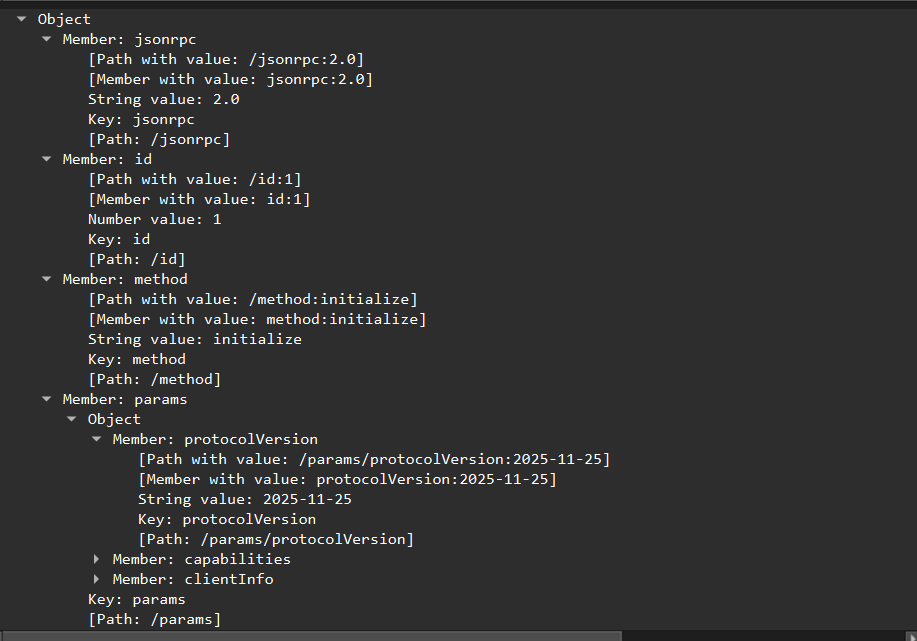
\includegraphics[width=0.74\textwidth]{03_initialize_request.png}
\vspace{0.4cm}
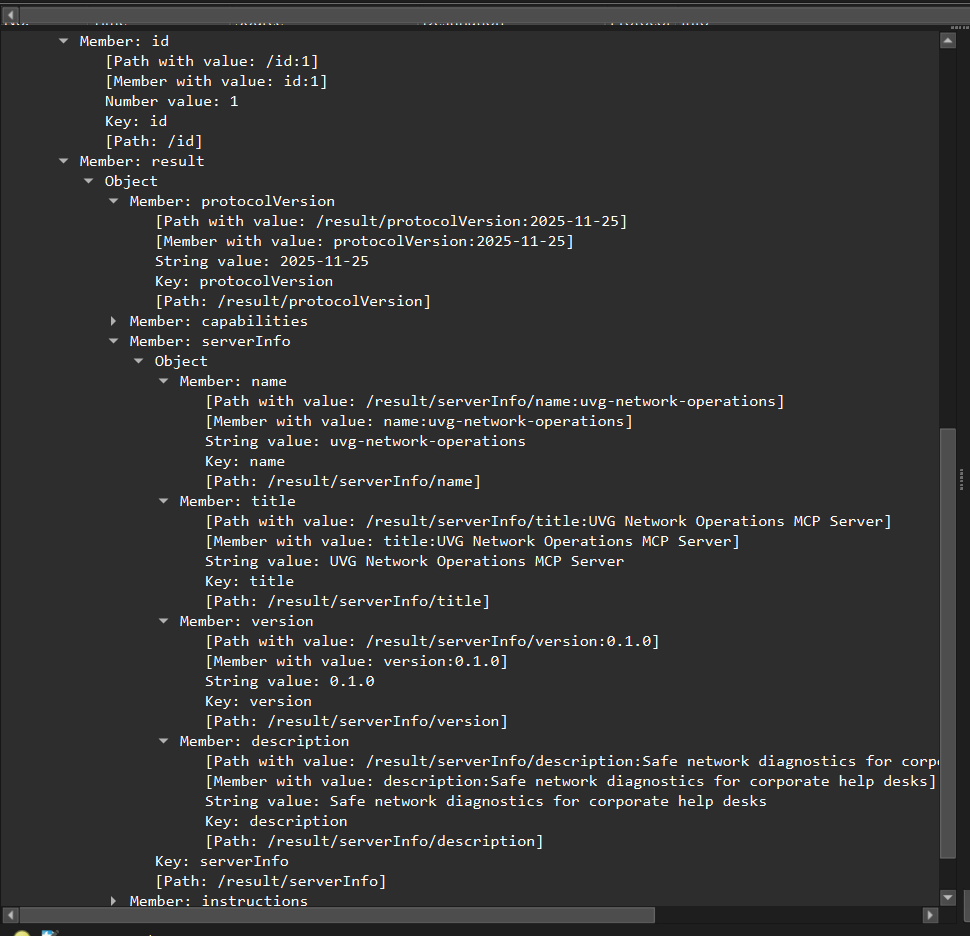
\includegraphics[width=0.74\textwidth]{04_initialize_response.png}
\caption{Solicitud y respuesta de inicialización}
\end{figure}

\begin{figure}[H]
\centering
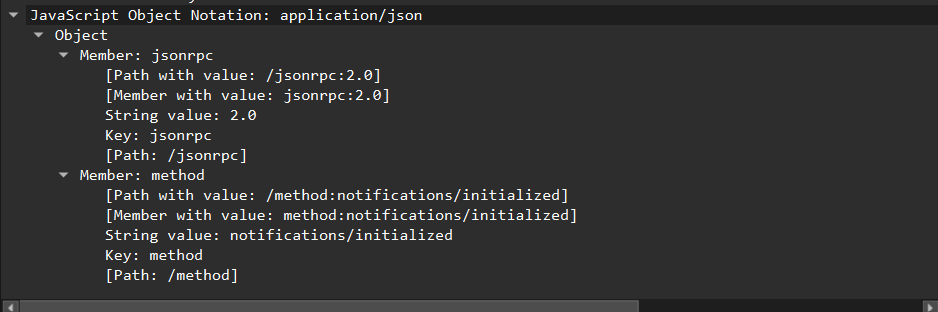
\includegraphics[width=0.60\textwidth]{05_initialized_notification.png}
\caption{Notificación de inicialización sin identificador}
\end{figure}

\subsection{Descubrimiento y ejecución}

La solicitud tools/list obtiene los nombres, descripciones y esquemas de las cuatro herramientas. La solicitud tools/call ejecuta una herramienta con argumentos validados y conserva el identificador en la respuesta.

\begin{figure}[H]
\centering
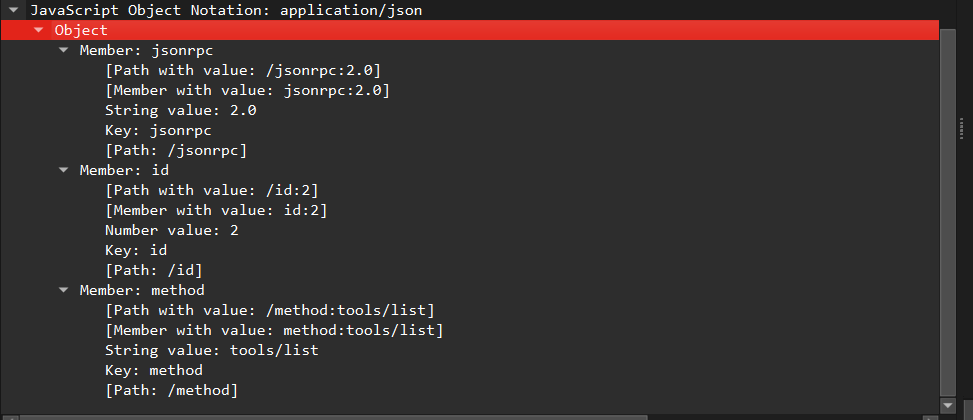
\includegraphics[width=0.60\textwidth]{06_tools_list_request.png}
\vspace{0.4cm}
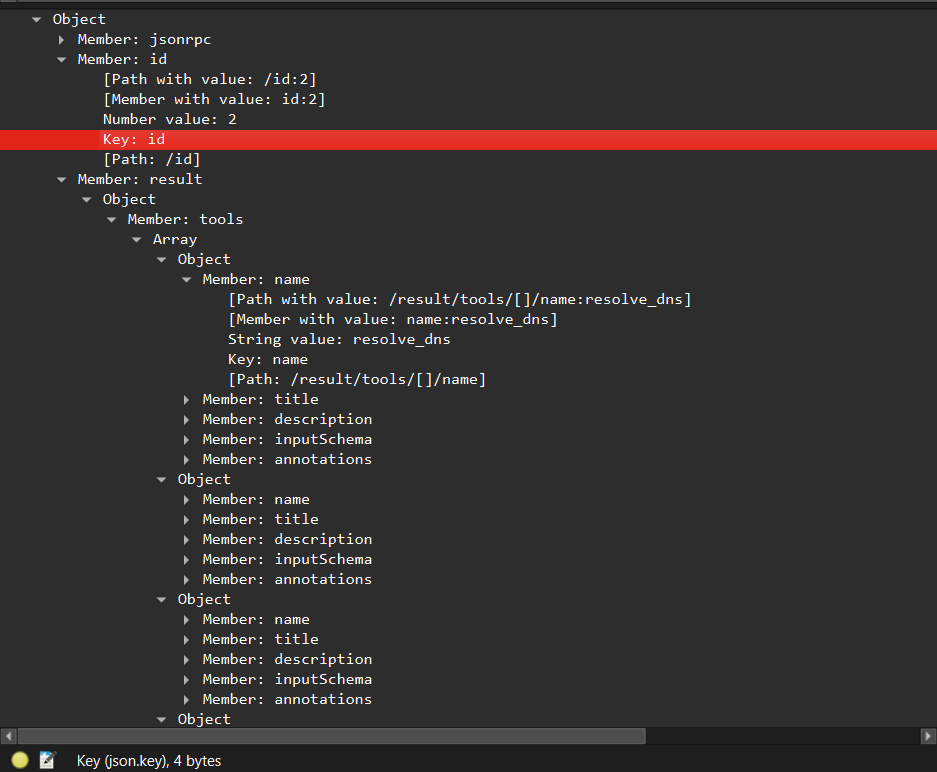
\includegraphics[width=0.60\textwidth]{07_tools_list_response.png}
\caption{Solicitud y respuesta del descubrimiento de herramientas}
\end{figure}

\begin{figure}[H]
\centering
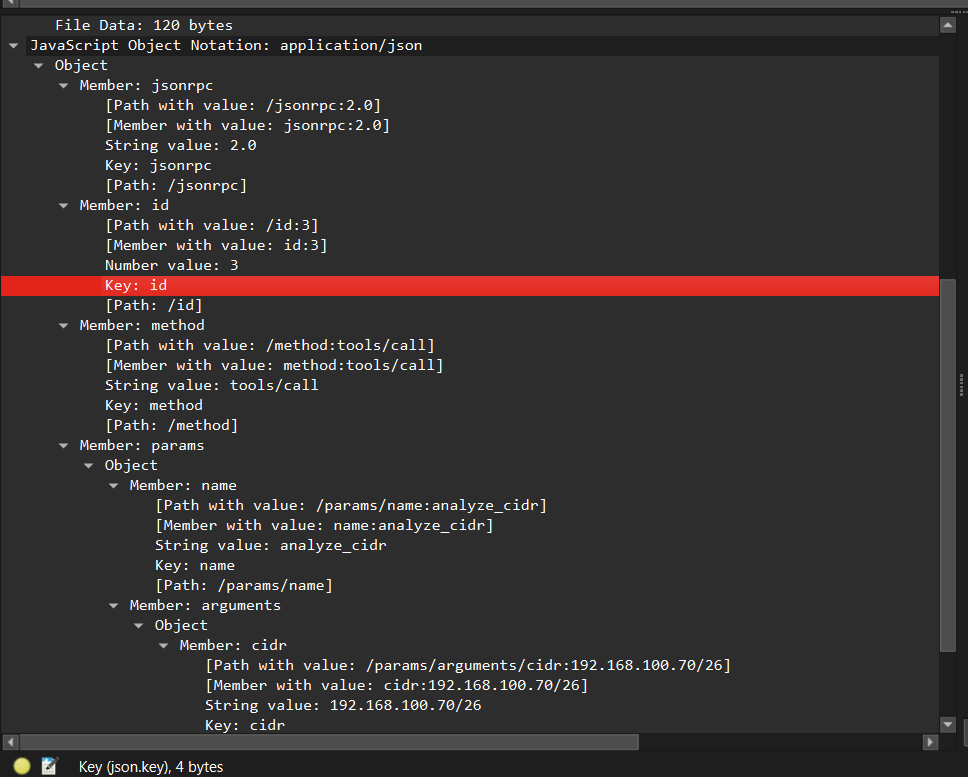
\includegraphics[width=0.76\textwidth]{08_tool_call_request.png}
\vspace{0.4cm}
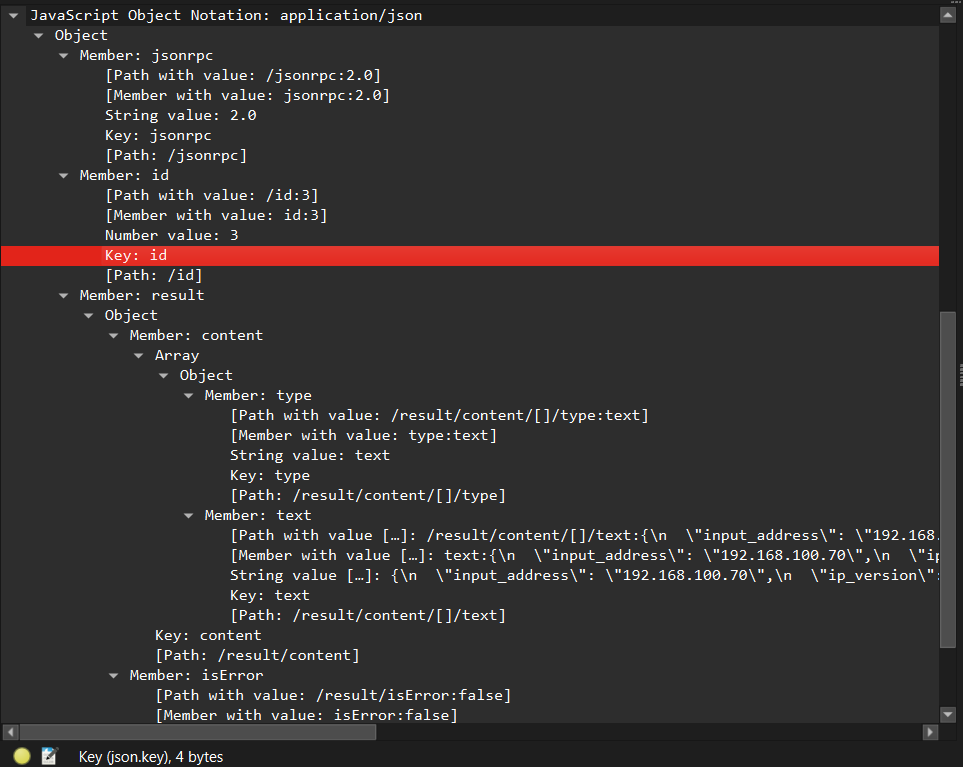
\includegraphics[width=0.76\textwidth]{09_tool_call_response.png}
\caption{Solicitud y respuesta de la ejecución de una herramienta}
\end{figure}

\section{Pruebas y resultados}

La suite automatizada finalizó con 16 pruebas aprobadas. Se validaron los esquemas del servidor, el transporte local, el transporte HTTP, la autenticación, la versión del protocolo, el contexto de Gemini, los reintentos y la selección de herramientas.

Las verificaciones manuales confirmaron el health check de Render, el descubrimiento de cuatro herramientas, la ejecución remota autenticada, la integración con Filesystem y Git y una conversación con contexto. El flujo Gemini hacia el servidor remoto analizó 172.16.5.130/26 y devolvió la red 172.16.5.128, el broadcast 172.16.5.191 y el rango útil 172.16.5.129 a 172.16.5.190.

\section{Conclusiones}

MCP permitió separar el modelo, el anfitrión y las herramientas mediante un contrato común. La implementación manual facilitó distinguir solicitudes, respuestas y notificaciones, además de comprender la función de los identificadores JSON-RPC.

El servidor local y el servidor remoto ofrecen las mismas herramientas sin cambiar su contrato. Esto demuestra que MCP permite cambiar el transporte sin modificar la lógica de negocio. El despliegue remoto agregó autenticación, TLS, health checks y validaciones propias de un servicio real.

Wireshark permitió relacionar MCP con Ethernet, IPv4, TCP, TLS y HTTP. La captura mostró la sincronización, el descubrimiento de herramientas y una ejecución exitosa. Las pruebas y las validaciones reales confirmaron que la solución cumple los objetivos del proyecto.

\section{Referencias}

\begin{itemize}
    \item \href{https://modelcontextprotocol.io/specification/2025-11-25}{Model Context Protocol. Specification 2025-11-25}
    \item \href{https://www.jsonrpc.org/specification}{JSON-RPC Working Group. JSON-RPC 2.0 Specification}
    \item \href{https://ai.google.dev/gemini-api/docs/function-calling}{Google AI for Developers. Gemini API Function Calling}
    \item \href{https://render.com/docs/infrastructure-as-code}{Render. Blueprints Infrastructure as Code}
    \item \href{https://www.wireshark.org/docs/wsug_html_chunked/}{Wireshark Foundation. Wireshark User Guide}
\end{itemize}

\end{document}
